
\newpage
\section{Results}

This chapter presents the outcomes of the design-based research (DBR) process, focusing on the iterative development and evaluation of the XR drone simulation system.

An initial attempt was made to implement drone physics directly in WebXR. However, the preliminary results revealed significant limitations in terms of stability. As a result, the approach was revised, and an existing FPV drone physics model \parencite{yuetility2022fpvphysics} was adopted to support subsequent iterations.

The chapter is structured into three main components: (1) the preliminary implementation of WebXR drone physics, (2) the iterative development of XR interaction, and (3) the iterative development of the Human-AI collaboration agent. Each component is presented following iterative cycles of design, enactment, analysis, and redesign, in accordance with the DBR framework as illustrated in \cref{fig:dbr_cycle}.

% Object: Drone Physics
\subsection{Preliminary Iteration: WebXR Drone Physics Implementation}

\paragraph{Design}

In the initial design iteration, the implementation of drone physics was simplified. Unlike full physical modeling of multi-rotor dynamics, including clockwise (CW) and counter-clockwise (CCW) torque balancing as described in \cref{eq:torque}, the first prototype adopted a simplified physics representation.

The drone object was implemented in the Wonderland Engine using the PhysX system provided by NVIDIA. A box collider was used as the primary collision shape, ensuring basic physical interaction with the environment. The system included two primary state variables: appliedForce and appliedTorque, which were updated in each frame within the update loop. User input was processed through a custom ReadInput function that retrieved joystick values from the WebXR input API, due to the lack of native input profile configuration support in the Wonderland Engine. The drone object design is illustrated in \cref{fig:webxr_drone}.

\begin{figure}[H]
    \caption{Components of the drone Object}\label{fig:webxr_drone}
    \centering
\begin{tikzpicture}

\umlclass[x=0, y=0]{DroneObject}{
  - appliedForce : float \\
  - appliedTorqueYaw : float \\
  - appliedTorqueRoll: float \\
  - appliedTorquePitch: float \\
  \dots
}{
  + Update() : void \\
  + ReadInput() : void
}

\umlclass[x=6, y=2]{PhysXComponent}{
  + shape : Box \\
  + engine : NVIDIA PhysX
}{
}

\umlclass[x=6, y=-2]{CollisionComponent}{
      + shape : Box 
}{
}

\umluniassoc{DroneObject}{PhysXComponent}
\umluniassoc{DroneObject}{CollisionComponent}

\end{tikzpicture}
\end{figure}


\paragraph{Enactment}

During implementation, the system was able to run in a WebXR environment; however, unstable flight behavior was observed. In particular, the drone exhibited oscillatory motion during navigation, and the tuning of applied torque parameters did not produce consistent control behavior.

\begin{figure}[H]
    \caption{Preliminary implementation of drone physics in WebXR}\label{fig:webxr}
    \centering
    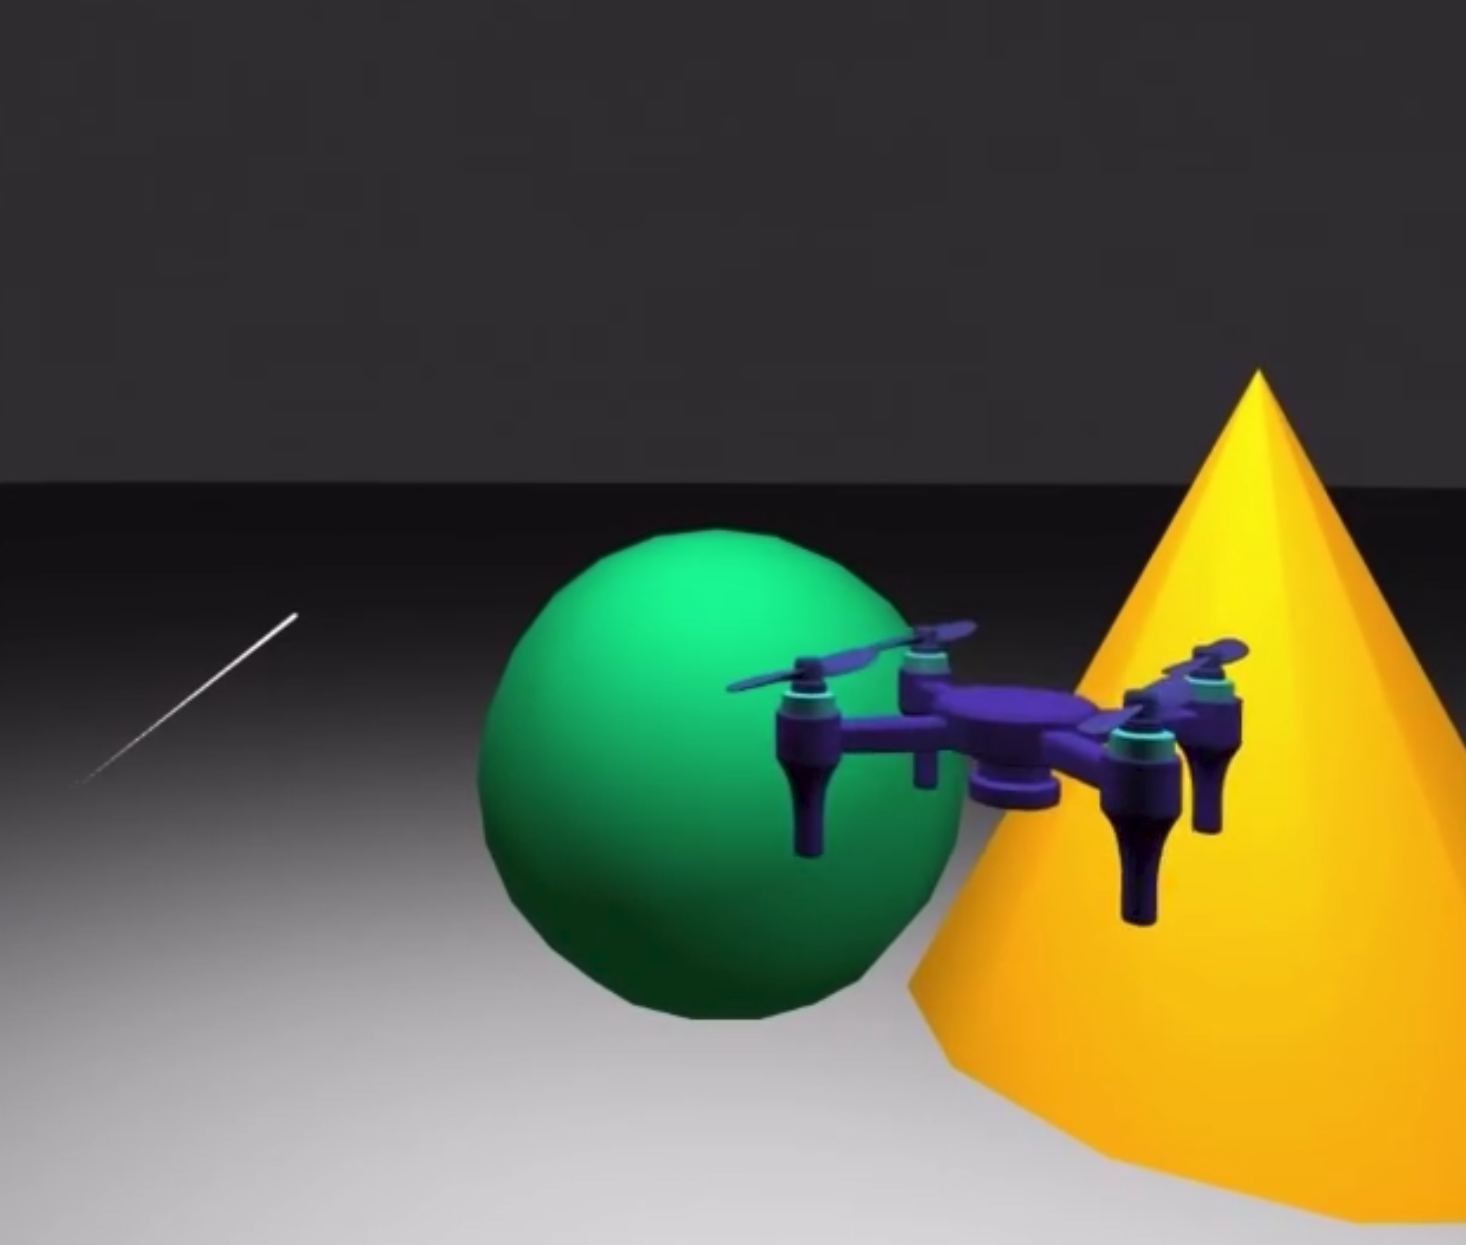
\includegraphics[width=0.6\linewidth]{img/webxr.png}
\end{figure}

The cause of these issues could not be conclusively identified within this iteration. Potential factors include limitations in browser-based physics execution, instability in the WebXR runtime environment, or insufficient documentation and debugging support in the Wonderland Engine.

As a result, alternative development platforms were explored. Microsoft AirSim \parencite{shah_airsim_2017}, built on Unreal Engine, was initially considered due to its advanced simulation capabilities. However, hardware constraints on the development machine limited its feasibility for continued development.

Following this evaluation, the study transitioned to the FPV drone physics model proposed by \parencite{yuetility2022fpvphysics}, implemented in Unity, as a more stable and extensible solution for subsequent iterations.

\paragraph{Analysis}

This preliminary iteration highlights the importance of selecting a suitable development engine for physics simulation in XR environments. Based on these findings, the subsequent methodology phase with a comparative evaluation of available development engines to ensure system stability and development feasibility.

\subsection{Iterative Development of XR interaction}
% XR interactions
\subsubsection{Iteration 1: Basic XR Control}

The architecture of Yue's ultimate drone physics shown in \cref{fig:quad_structure}. A quad GameObject includes (1) Rigidbody, Unity's physics (2) YueInputModule, used to calculate controller axis. (3) YueDronePhysics, used to calculate the physics should applied on the drone's body with YueInputModule. (4) DroneXrEmulator, Map the Meta Quest Touch controller joystick data to YueInputModule.

\begin{figure}[h]
    \caption{The Components of the Quad GameObject}\label{fig:quad_structure}
    \centering
    \[
    \begin{array}{|c|}
    \hline
    \mathbf{GameObject: Quad} \\
    \hline
    \text{Rigidbody} \\
    \text{YueInputModule} \\
    \text{YueDronePhysics} \\
    \text{DroneXrEmulator} \\
    \hline
    \end{array}
    \]
\end{figure}


To implement video passthrough, The scene should include the AR session into the scene, also add AR Raycast manager into the XR Origin. And add “AR Camera Manager” and “AR Camera background” on the MainCamera. 

The result as shown in \cref{fig:drone-in-xr}

\begin{figure}[H]
    \caption{Controlling the drone physics in XR environment}\label{fig:drone-in-xr}
    \centering
    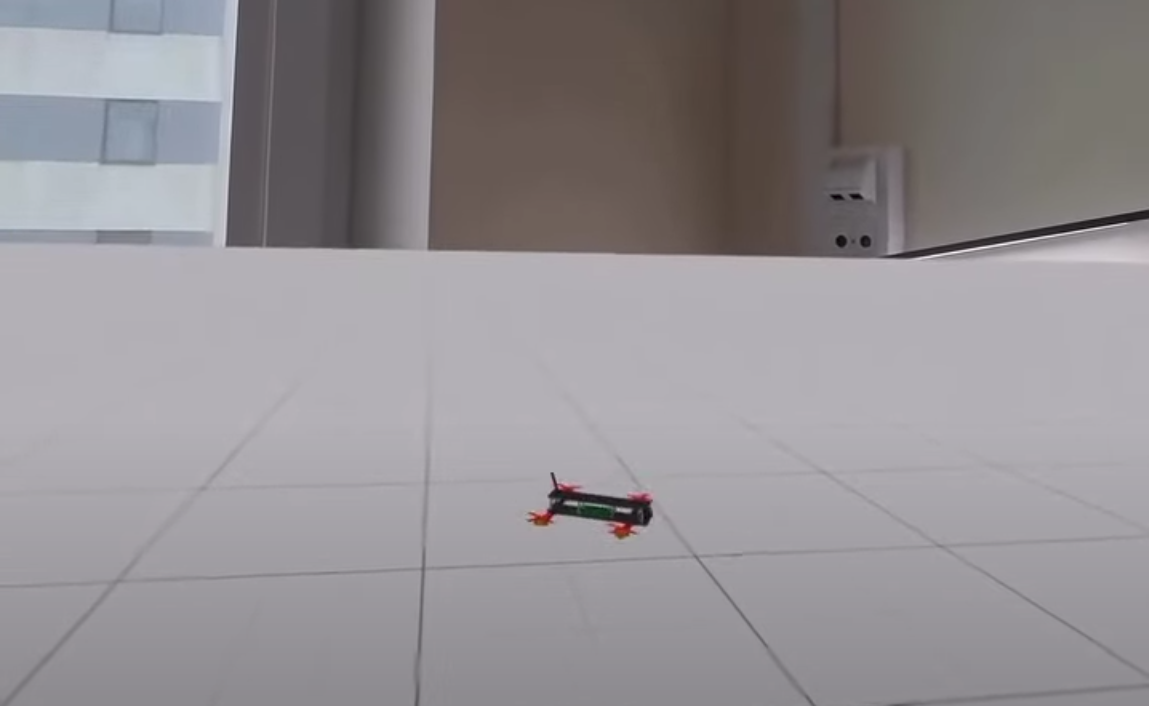
\includegraphics[width=0.8\linewidth]{img/stages/drone-control.png}
\end{figure}
\subsubsection{Iteration 2: Supporting Learning through UI and Tutorial}

\paragraph{Design}

The findings from the previous iteration indicated that participants were initially unable to understand the controller-based interaction. Therefore, this iteration focused on improving learnability through structured tutorials, enhanced visual feedback, and environmental constraints.

The system was extended with three primary interaction components: (1) the Quad GameObject, representing the physical quadcopter model; (2) the DroneVision GameObject, which uses Unity's RenderTexture to provide a first-person view (FPV) through a virtual headset; and (3) the Instruct GameObject, which delivers step-by-step tutorial guidance. The structure of the scene is illustrated in \cref{fig:tutorial_scene}.

\begin{figure}[H]
    \caption{Components of the Tutorial Scene}\label{fig:tutorial_scene}
    \centering
    \begin{tikzpicture}
        % 建议先定义类，再用 umlpackage 包含，或确保坐标明确
        \begin{umlpackage}{Tutorial Scene}
            \umlclass[width=3cm]{Quad}{
                + FpvCam: Camera
            }{
            }
            
            \umlclass[x=6, width=4cm]{DroneVision}{
                - renderTexture : RenderTexture
            }{}
            
            \umlclass[y=-3, x=3, width=4cm]{Instruct}{
                - tutorialSteps : List
            }{
                + Next()
            }
            
            % 连线需放在 package 内部或紧随其后
            \umluniassoc{DroneVision}{Quad}
            \umluniassoc{Instruct}{Quad}
            \umluniassoc{Instruct}{DroneVision}
        \end{umlpackage}
    \end{tikzpicture}
\end{figure}

The Quad GameObject functions as the physical simulation of the quadcopter, while DroneVision renders the onboard camera feed to simulate FPV piloting. The Instruct module presents content in a sequential manner, covering arming, throttle, yaw, pitch, and roll control. During tutorial execution, the quadcopter's Rigidbody is temporarily locked to support reflective observation, consistent with Kolb's experiential learning cycle \parencite{kolb1984}.

To improve interaction awareness, a dual-layer HUD system was introduced. A cross-axis indicator was rendered in front of the player, while corresponding visual markers were placed within the scene to represent real-time joystick input positions.

In total, six interaction modes were implemented. Five correspond to quadcopter flight control in mode 2 \cref{fig:mode2}, while one supports general XR interaction:

\begin{itemize}
    \item \textbf{Arm}: Activates the rotor system by pulling the left joystick to its minimum position.
    \item \textbf{Throttle}: Controls vertical thrust by adjusting the vertical axis of the left joystick.
    \item \textbf{Yaw}: Controls rotational movement around the vertical axis via horizontal movement of the left joystick.
    \item \textbf{Pitch}: Controls forward and backward tilt using the vertical axis of the right joystick.
    \item \textbf{Roll}: Controls lateral tilt using the horizontal axis of the right joystick.
    \item \textbf{Grip/Select}: Enables interaction with UI elements using the controller grip button.
\end{itemize}

Additionally, the DroneXrEmulator \cref{fig:quad_structure} was extended with a BoxCollider parameter to define a bounded safe flight area.

\paragraph{Enactment}

The updated system maintained a video-passthrough XR environment while introducing structured abstractions that map directly to real-world drone control inputs. The tutorial system guided users through incremental interaction learning, while the HUD provided continuous feedback of controller input states. The inclusion of a bounded flight space ensured that users remained within a safe operational area during early learning stages.

\begin{figure}[H]
    \caption{Structure of the interaction system components}\label{fig:interact}
    \centering
    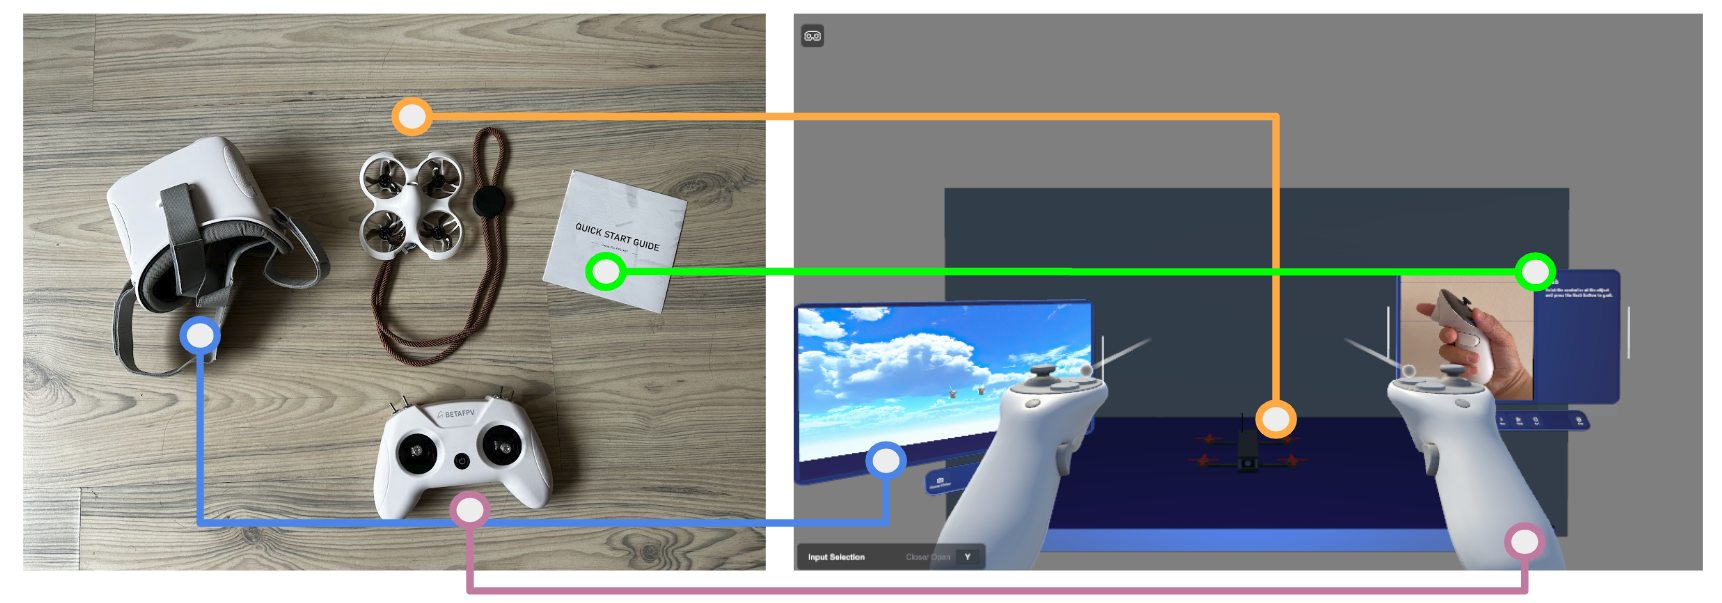
\includegraphics[width=0.8\linewidth]{img/stages/structure.png}
\end{figure}

\paragraph{Analysis}

Observational testing showed that participants were able to understand basic controller interactions in third-person mode after the introduction of the tutorial system. However, difficulties persisted in spatial orientation during FPV (DroneVision) mode. In particular, the skydome environment did not provide sufficient directional cues, which negatively impacted navigation performance in first-person piloting scenarios.
\subsubsection{Iteration 3: Test Flight in a Realistic Environment}

\paragraph{Redesign}

Findings from the previous iteration indicated that users experienced difficulty in maintaining spatial orientation during first-person flight. The skybox environment did not provide sufficient visual cues for direction perception.

To address this limitation, a realistic urban environment was introduced. Based on publicly available datasets \parencite{TallinnCityModel2012, EstonianLandBoard2020}, a 3D model of Tallinn was imported into Unity to construct the simulation environment (see \cref{fig:tallinn}).

Within this environment, a goal-oriented task was designed in which the player navigates from Viru Gate to Tallinn Town Hall. Directional signs and collectible elements (e.g., coins) were implemented to provide guidance and reinforce goal-directed navigation.

\paragraph{Enactment}

The imported city model and terrain are shown in \cref{fig:tallinn}. To ensure real-time performance in XR, occlusion culling was applied to reduce rendering load by excluding non-visible geometry.

\begin{figure}[H]
    \caption{The Tallinn Old Town model (top) and terrain (bottom) imported into Unity}\label{fig:tallinn}
    \centering
    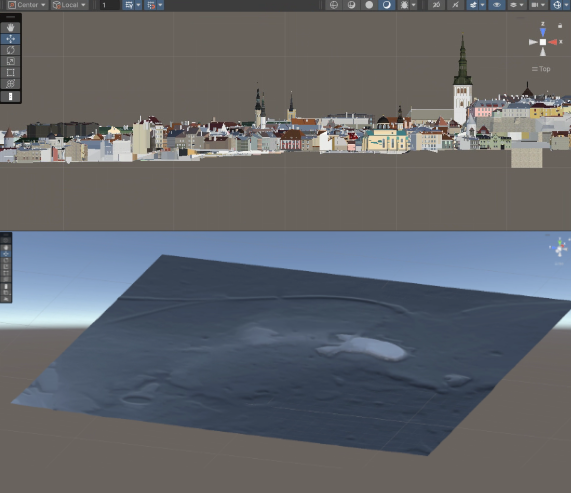
\includegraphics[width=0.6\linewidth]{img/Tallinn.png}
\end{figure}

After refinement of the skybox and building materials, the final environment is presented in \cref{fig:realistic}, including the navigation route, player view, collectible elements, and mesh-based collision boundaries.

\begin{figure}[H]
    \caption{Navigation route in the green collider (top), player view (bottom-left), and coin collection with mesh collider (bottom-right)}\label{fig:realistic}
    \centering
    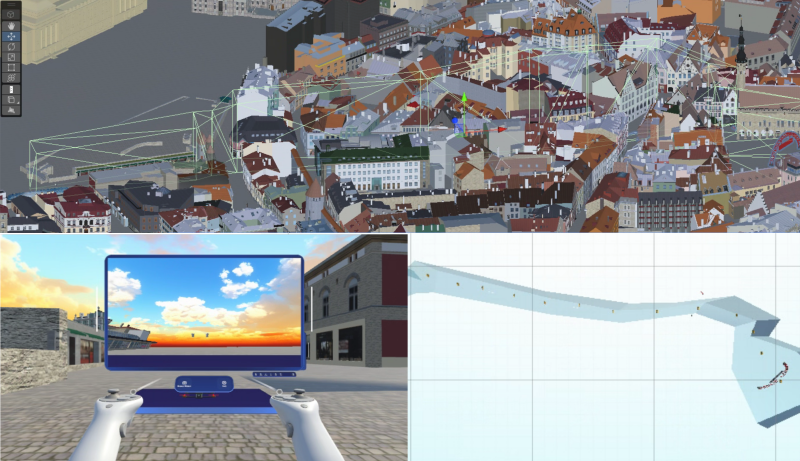
\includegraphics[width=0.6\linewidth]{img/real.png}
\end{figure}

\paragraph{Analysis}

The introduction of a realistic environment significantly enhanced user engagement and perceived immersion. Play tests shows that the enriched visual context improved their ability to orient themselves during flight.

Some participants suggested enabling free exploration of the environment, aligning with the active experimentation stage of experiential learning.

At the same time, the increased visual complexity led to performance challenges in XR rendering. Several testers proposed the use of simplified or white-box environments to lower down the performance issue.
\subsubsection{Iteration 4: Downgraded White-Box Playground}

\paragraph{Redesign}

In the previous iteration, performance limitations of the target device were identified as a critical constraint. To address this issue, the realistic city environment was removed. The redesigned environment retains only essential elements, including collision boundaries and a predefined flight route, to support the goal-directed navigation.

\paragraph{Enactment}

As illustrated in \cref{fig:white-box}, the player operates the quadcopter within a simplified white-box environment. This environment consists of minimal visual features, focusing on spatial structure and navigational constraints rather than visual realism.

\begin{figure}[H]
\caption{Player controlling the quadcopter in a white-box playground}
\label{fig:white-box}
\centering
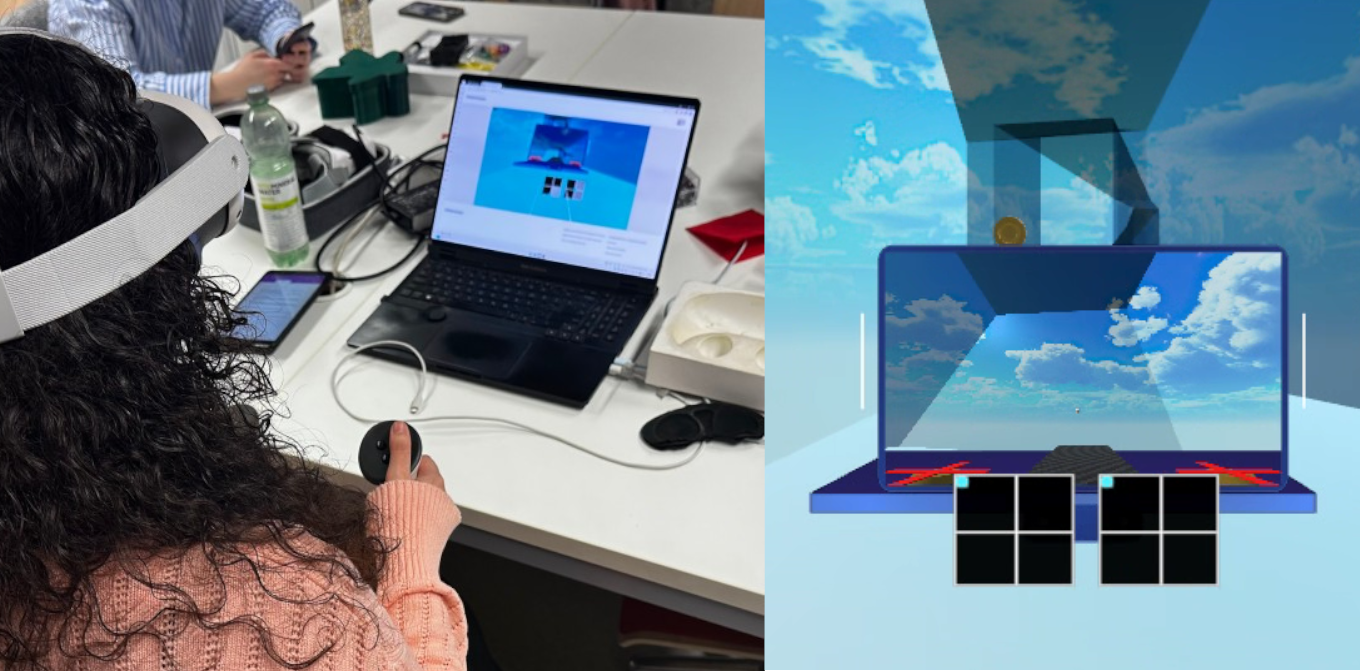
\includegraphics[width=0.8\linewidth]{img/white-box.png}
\end{figure}

\paragraph{Analysis}

The simplified environment is expected to improve system performance and provide a more stable interaction experience. However, user testing has not yet been conducted due to time constraints. Future evaluation is required to assess its effectiveness.

% TODO: Need test play, only 3 days left!!!!

\subsubsection{Iteration 5: Exploration in a Realistic Environment}

\paragraph{Redesign}

Building on the third iteration, an exploration mode within a realistic environment was introduced to support the active experimentation stage of experiential learning. The aim was to enable users to navigate the environment more freely and apply previously acquired piloting skills in a less constrained context.

To evaluate this approach, environmental constraints were reduced by removing collider boundaries. Participants were assigned a navigation task requiring them to travel independently from Viru Gate to St.\ Olaf's Church, the tallest structure in the modeled environment (see \cref{fig:tallinn}).

\paragraph{Enactment}

The technical modification involved the removal of boundary constraints, without introducing additional interaction mechanics.

Due to the absence of colliders, the quadcopter was able to pass through building meshes. Additionally, as the drone increased in altitude, a larger number of buildings were rendered in the scene, which led to a decrease in frame rate and negatively affected the user experience.

However, the immersive environment appeared to encourage exploration. Users tended to engage for longer periods compared to previous iterations, as the absence of failure conditions (e.g., crashes) reduced frustration.

\paragraph{Analysis}

The results suggest that an immersive environment may increase user engagement and practice duration. Furthermore, reducing failure conditions appears to lower user frustration.

However, it remains unclear whether these changes lead to measurable improvements in learning outcomes. Future work should incorporate quantitative data collection and comparative analysis to evaluate the effectiveness of this approach.


% AI for learning
\subsection{Iterative Development of Human-AI Collaboration Agent}

\subsection{Path Following with PID Controller}

It is better to complete this section in a flat panel display. As this part is more algorithm centered. Instead of using the DroneXrEmulator in \cref{fig:quad_structure}, it is simpler to make another PidDroneEmulator which maps the calculated joystick value to YueInputModule.

To implement path following, two other components are included, PathFollower, cut the path into different targets for PidDroneEmulator to calculate errors and PathGenerator to build the path.

To move between points, the PathGenerator generates a path using two Cubic Bézier curves. Given four control points $P_0, P_1, P_2, P_3$, home to waypoint and back, the position $B(t)$ for $t \in [0,1]$ is defined as \cref{eq:bezier}.

\begin{equation}\label{eq:bezier}
    B(t) = {(1-t)}^3 P_0 + 3{(1-t)}^2 t P_1 + 3(1-t) t^2 P_2 + t^3 P_3
\end{equation}

The path is constructed relative to the Home and Target vectors, the drone will fly from Home and fly back, the path as shown in \cref{fig:path_design}. Path from Home to Waypoint using a right-hand offset for control points; Path from Waypoint back to Home using a left-hand offset.

\begin{figure}[H]
    \caption{Path Design}\label{fig:path_design}
    \centering
    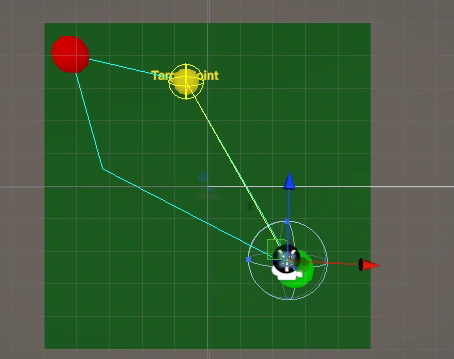
\includegraphics[width=0.8\linewidth]{img/path.png}
\end{figure}

By calculating these normalized joystick rates, the system can visualize the AI's calculation on the HUD.This serves as an AI collaboration hinter, showing human pilots the optimal stick positions for maintaining the designated path \cref{fig:pid-ui}.

\begin{figure}[H]
    \caption{hinter UI}\label{fig:pid-ui}
    \centering
    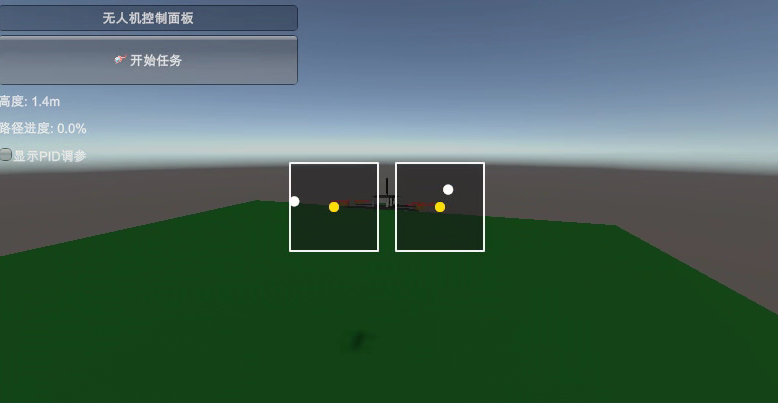
\includegraphics[width=0.8\linewidth]{img/ui.png}
\end{figure}


\subsubsection{Iteration 2: Exploration of RL-Based Control (Preliminary)}

This iteration explored the use of a reinforcement learning (RL) agent for hovering control. The goal was to reduce the high-frequency control signals observed in the PID-based approach and provide smoother guidance that better matches human perception.

\paragraph{Design}

A simplified 1D hovering task was implemented, where the agent controlled the vertical position ($y$) to stay within a target band $[H - R, H + R]$. The agent received two observations: a normalized height error and the vertical velocity. A reward function combining event-based and continuous feedback was used to encourage stable hovering behavior.

The agent was trained using Proximal Policy Optimization (PPO) for $5 \times 10^5$ steps. Training progress was monitored through cumulative reward and episode length.

\paragraph{Enactment}

The machine learning process was implemented using Unity's ML-Agents toolkit, which leverages PyTorch as its underlying deep learning framework and provides training analytics for performance evaluation. The results indicate that the agent successfully learned to maintain stable hovering within the designated target range. As shown in Figure~\ref{fig:rl_result}, the cumulative reward increased steadily after approximately 100,000 training steps and plateaued around 400,000 steps. Furthermore, episode length progressively increased over time, suggesting improved flight stability and control performance.

\begin{figure}[H]
    \caption{Training performance of the reinforcement learning agent using PyTorch via Unity ML-Agents.}\label{fig:rl_result}
    \centering
    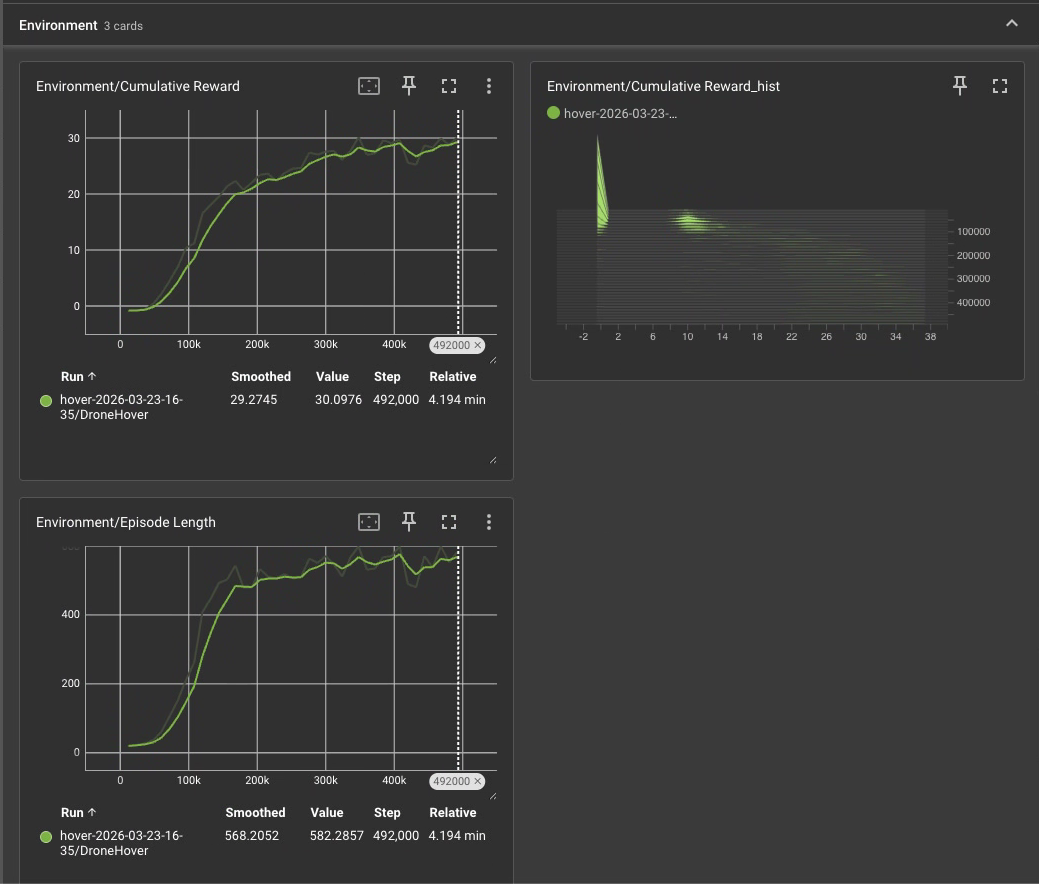
\includegraphics[width=1\linewidth]{img/result.png}
\end{figure}

Moreover, the use of a decision interval (DecisionRequester) enabled the control output to be updated at a lower frequency, resulting in smoother control signals compared to the PID-based approach, which aligns more closely with human perceptual capabilities (see Figure~\ref{fig:rl_hover}).

\begin{figure}[H]
    \caption{User interface prototype of the reinforcement learning agent.}\label{fig:rl_hover}
    \centering
    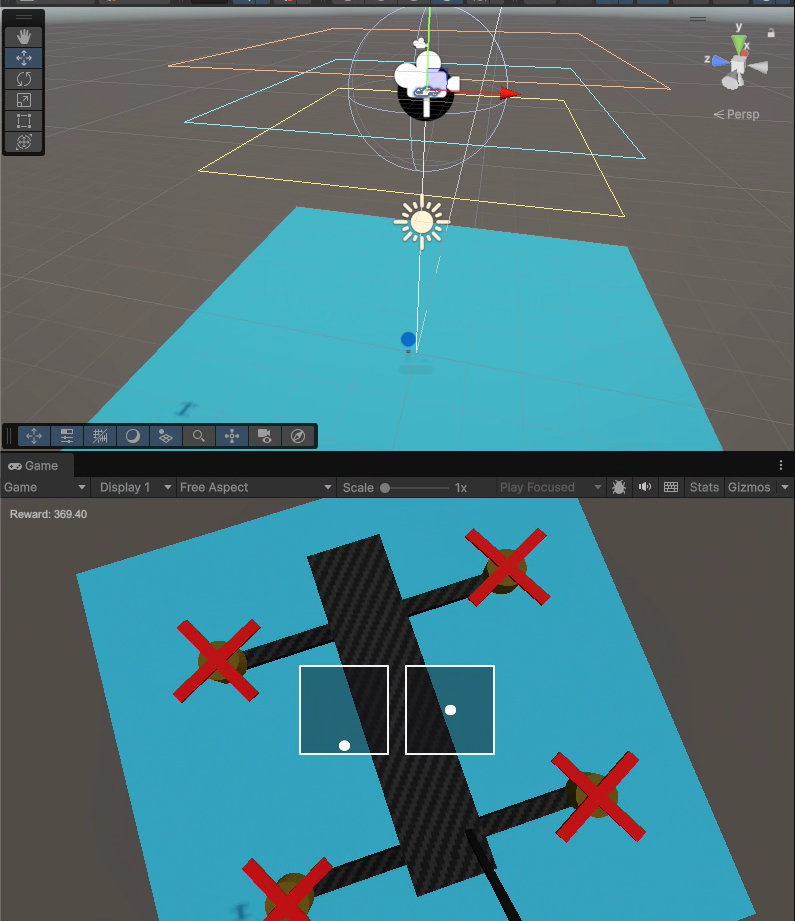
\includegraphics[width=1\linewidth]{img/hover.png}
\end{figure}

\paragraph{Analysis}

Although the RL agent achieved stable hovering in a simplified setting, several limitations were identified.

First, the approach did not scale well to more complex tasks such as path following. These tasks require a larger set of state variables (e.g., position, velocity, and angular motion in multiple axes), which increases the difficulty of training.

Second, the RL model behaved as a black-box system. Fine-tuning the behavior required extensive experimentation, and the relationship between parameters and performance was difficult to interpret.

Third, compared to the PID-based method, the RL approach required significantly more training time and computational resources, while not providing a clear advantage in control stability in the current study.

The RL-based approach is considered promising for future work. However, it requires a more systematic pipeline, such as data collection and state variable reduction (e.g., using principal component analysis), which is beyond the scope of the current study.
\subsubsection{Iteration 3: Evaluation on Hovering Task}

This iteration focused on refining the PID controller and evaluating its performance in a hovering task.

\paragraph{Design}

To improve controller stability, the joystick update interval was adjusted to one update every 20 frames. In addition, the PID parameters were fine-tuned, as presented in \cref{table:pid_params}.

\begin{table}[h]
\centering
\caption{PID Controller Parameters} \label{table:pid_params}
\begin{tabular}{lccccc}
\hline
\textbf{Controller} & \textbf{Axis} & $K_p$ & $K_i$ & $K_d$ & Max Output \\
\hline
Position (Outer Loop) & X & 2.0 & 0.10 & 1.5 & 10 \\
Position (Outer Loop) & Y & 3.0 & 0.12 & 1.5 & 15 \\
Position (Outer Loop) & Z & 2.0 & 0.10 & 1.5 & 10 \\
\hline
Velocity (Inner Loop) & X & 1.0 & 0.05 & 0.3 & 8 \\
Velocity (Inner Loop) & Y & 1.5 & 0.10 & 0.5 & 12 \\
Velocity (Inner Loop) & Z & 1.0 & 0.05 & 0.3 & 8 \\
\hline
Yaw Control & Yaw & 3.0 & 0.00 & 1.0 & 5 \\
\hline
\end{tabular}
\end{table}

\paragraph{Enactment}

In the hovering task, the refined PID controller produced stable performance. As illustrated in \cref{fig:rl_hover}, both the PID controller (orange) and the RL agent (blue) were tasked with maintaining a constant altitude of 5 meters. Data were collected over a duration of 60 seconds. The results indicate that the PID controller maintained a stable hover, whereas the RL agent exhibited greater oscillation around the target height.

\begin{figure}[H]
    \caption{Hovering task results. The top plot shows throttle input, and the bottom plot shows drone altitude.}\label{fig:rl_hover}
    \centering
    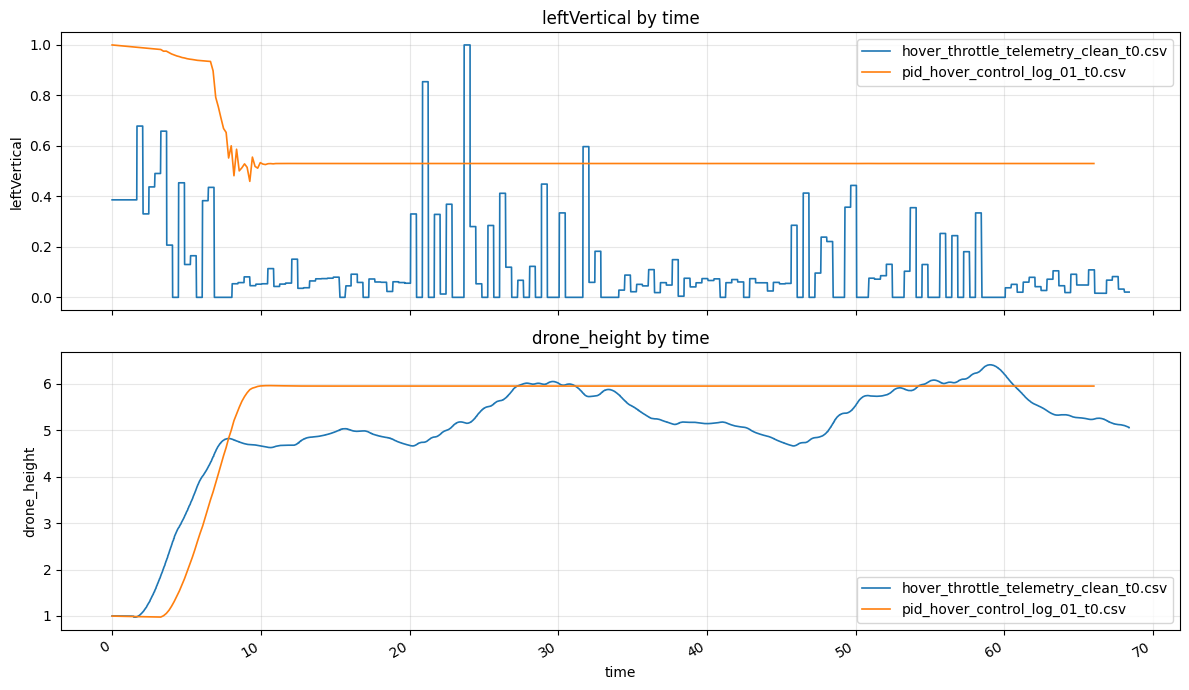
\includegraphics[width=0.8\linewidth]{img/result_hovering.png}
\end{figure}

\paragraph{Analysis}

After parameter tuning, the PID controller demonstrated stable and reliable altitude control in the hovering task. This level of performance was considered sufficient to proceed to the subsequent path-following evaluation.
\subsubsection{Iteration 4: Evaluation on Path Following}

In this iteration, the drone was designed to follow a predefined path consisting of three sequential stages: take-off to a target altitude, navigation to a designated waypoint, and return to the home position, as described in the evaluation strategy in \cref{fig:path_design}. A cascading PID control structure was applied.

\paragraph{Design}

During the execution of the path-following task, the drone's position, rotation, and raw joystick inputs were recorded. The evaluation focuses on four visual analyses: (1) jerk magnitude over time, defined as the time derivative of acceleration and computed as $J = \sqrt{j_x^2 + j_y^2 + j_z^2}$, to assess motion smoothness; (2) throttle and pitch signals over time to examine forward flight behavior; (3) yaw and roll signals over time to evaluate turning behavior; and (4) a 3D trajectory plot to verify whether the intended path was successfully followed.

\paragraph{Enactment}

The results are shown in \cref{fig:path_result}. The left figure illustrates the full trajectory of the drone, including take-off, navigation to the waypoint, and return to the home position. From top to bottom, the subplots present: jerk magnitude over time; throttle (blue) and pitch (orange) joystick inputs over time; and yaw (blue) and roll (green) inputs over time.

\begin{figure}[H]
    \caption{Path Following Task Result.}\label{fig:path_result}
    \centering
    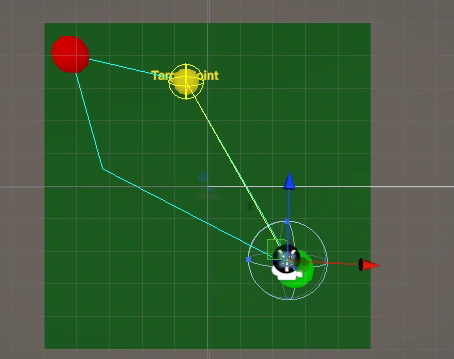
\includegraphics[width=1\linewidth]{img/path.png}
\end{figure}

\paragraph{Analysis}

As observed in the results in \cref{fig:path_result}, consistent with the previous iteration, the controller performs well during take-off and hovering phases. However, during forward flight, the pitch signal exhibits noticeable instability, occasionally taking negative values, indicating unintended backward motion. A similar issue can be seen during turning behavior, the bottom graph, where yaw and roll signals show inconsistent and negatively correlated patterns, whereas a positively correlated relationship would be expected under stable coordinated control.

Despite these instabilities, the system demonstrates sufficient functional performance for integration with the XR environment at its current stage of development.

\subsection{Integration: Human-AI Collaboration in an XR Environment}

Building on the XR environment and the human-AI collaboration agent developed in prior iterations, this iteration focuses on integrating these components into a unified system.

\paragraph{Design}

In the XR development iteration, a heads-up display (XrJoystickHud) was introduced to provide real-time feedback on the user's joystick inputs. In the iteration, this interface is extended to visualize the AI agent's suggested joystick actions, thereby enabling a direct comparison between user input and agent guidance.

To support this functionality, the structure of the XrJoystickHud was modified to receive data from two emulator components (DroneXrEmulator). One emulator maps joystick data from the XR environment to the YueInputModule (see \cref{fig:quad_structure}), while the other emulator (PidEmulator) retrieves joystick signals generated by the PID controller, as illustrated in \cref{fig:hud}.


\begin{figure}[H]
\caption{Structure of XrJoystickHud}\label{fig:hud}
\centering

\begin{tikzpicture}

% Classes
\umlclass[style={fill=white}, x=0, y=0]{XrJoystickHud}{
}{
  + update()
}

\umlclass[style={fill=white}, x=-7, y=-1]{DroneXrEmulator}{
}{
  + getJoyStickData()
}

\umlclass[style={fill=white}, x=7, y=-1]{PidEmulator}{
}{
  + getJoyStickData()
}

\umlclass[style={fill=white}, x=-3, y=-4]{YueInputModule}{
    + rawInputLeftHorizontal: float \\
    + rawInputLeftVertical: float
}{
}

\umlclass[style={fill=white}, x=3, y=-4]{PidController}{
    + kp: float \\
    + ki: float \\
    + kd: float
}{
}

% Relationships
\umluniassoc[arg1=fetches, pos1=0.5]{XrJoystickHud}{DroneXrEmulator}
\umluniassoc[arg1=fetches, pos1=0.5]{XrJoystickHud}{PidEmulator}

\umluniassoc[arg1=maps to, pos1=0.5]{DroneXrEmulator}{YueInputModule}
\umluniassoc[arg1=calculates for, pos1=0.5]{PidController}{PidEmulator}

\end{tikzpicture}
\end{figure}

\paragraph{Enactment}

% TODO: Insert screenshot and describe implementation (1 day remaining)

\paragraph{Analysis}

% TODO: Complete analysis of user interaction and system performance (1 day remaining)

